\chapter{Conclusion and Future Directions}
\label{chap:conclusion}
% Discussion: remaining challenges, the benefits in another fields than oncology

My dissertation contributes to a better toolbox for cancer proteogenomic and multi-omics characterization and generates insights into glioblastoma disease biology that will lead to novel therapeutic avenues. In \Cref{chap:mut-pipeline-qc}, we investigated the data harmonization using standardized data processing pipelines on establish bulk genomic sequencing technologies. Data harmonization is part of the critical infrastructure of large-scale multi-omics studies to ensure the generated datasets can be integrated with other data of interest and re-used by the research community. We showed that the data harmonization on Genomic Data Commons is applicable to various studies across cancer types. More importantly, the harmonized outputs do not significantly alter the downstream biological findings and interpretation. In the cases where technical artifacts are introduced, those artifacts are carefully characterized and documented. Pipelines on GDC have since been applied to more cancer projects. Other data commons of different data types are actively being developed, including Proteomic Data Commmons and Imaging Data Commons, by following the example set by GDC.

In \Cref{chap:ptmcosmos}, we developed a database, PTMcosmos, that collects the existing knowledge of post-translation modifications in cancer and used the integrated information of PTmcosmos to analyze the experiment datasets from Clinical Proteomic Tumor Analysis Consortium to showcase its potential values to the research community. We collected the proteomic datasets from CPTAC, a consoritum with the goal of proteogenomic multi-omics characterization of patient tumors across multiple cancer types. By harmonizing the CPTAC's mass spectrometry based global protein and PTM abundance measurements with existing supporting evidences of PTM sites, we were able to identify pan-cancer PTM dysregulation events that are not explained by the known upstream genetic alterations or associated with clinically relevant tumor subtypes. We also investigated the mutational impact on PTM through protein structure guided spatial clustering. Furthermore, the easy-to-use user interface of PTMcosmos brings such functionalities to the end user, allowing the broader research community to utilize the immense amount of new PTM information brought by CPTAC and the known functions and annotations of PTMs from the literature.

In \Cref{chap:cptac-gbm-discov}, we focused on the proteogenomic characterization of glioblastoma in a CPTAC study. During the data analysis, we utilized the ``toolbox'', where the genomic data were harmonized on GDC and PTM annotations were pulled from PTMcosmos. Our analysis contributes to the potential improvement of patient stratification and discovery of new therapeutic options. Using multi-omics clustering, we identified a subset of patients with mixed subtypes compared with traditional sequencing-based subtypes, who exhibit shortened overall survival. Phosphoproteomic data indicate that PLCG1 and PTPN11 act as a common signaling hub for multiple RTKs. Given the high RTK genetic alteration frequencies and eventual remission in GBM, a combined therapy targeting both RTKs and their shared signaling hub might be more effective. Using connectivity map approach, we identified some druggable targets based on the gene and protein signatures of GBM tumors. By integrating the bulk multi-omics with single cell transcriptomics, we dissected the tumor microenvironment and characterized the immune composition differences and the potential signaling transduction regulation. In sum, our findings bring new insights towards a better understanding of GBM and hopefully a better personalized treatment for GBM patients.

Undoubtedly, there are new set of challenges that call for an upgraded bioinformatics toolbox and better multi-omics integration. The function of many PTM sites remain unknown and there is a lack of systematic understanding of the PTM regulation across cancer types. GBM remains difficult to treat and the mechanism behind the eventual recurrence of the tumor is elusive. We will dive into these challenges and future directions below.


\section{New technologies call for new harmonization pipelines and data repositories}
% new pipelines for new technology
In the past decade, the single cell technologies have made great breakthroughs that they are more accessible for large scale multi-omics studies \cite{chappelll_voett:SingleCellMulti2018}. Particular for single cell transcriptomics technologies, it is now possible to profile the full gene expression of tens of thousands of human cells in a single cell, generating high dimension cell-by-gene expression matrices that take more spaces to store and more computational power to process. While the existing data repositories like GDC are able to host the single cell data, there has not been a standard way to let users explore and extract part of the datasets for their down downstream analysis. On the other hand, the bulk genomic datasets can be explored more easily through integration portals like cBioPortal \cite{ceramie_schultzn:CBioCancer2012,gaoj_schultzn:IntegrativeAnalysis2013}. Due to the high dimensionality of the single cell data (cell per sample per cohort), new innovations are required to redesign the user interface and visualization. More broadly speaking, new imaging based/assisted single cell technologies such as multiplexed imaging \cite{giesenc_bodenmillerb:HighlyMultiplexed2014,goltsevy_nolangp:DeepProfiling2018,tanwcc_limtkh:OverviewMultiplex2020} and spatial transcriptomics \cite{morrissa_morrissa:PinpointingSpatial2019,longosk_khavaripa:IntegratingSinglecell2021,driesr_yuangc:AdvancesSpatial2021} will bring in a new set of challenges to integrate the genomic data with imaging data.

Like bulk genomics data, data generated by the new technologies also requires a careful review and quality check of their data harmonization. For single cell transcriptome technologies, the data processing and integration methods are still under active development and lack consensus \cite{lahnemannd_schonhutha:ElevenGrand2020,andrewsts_hembergm:TutorialGuidelines2021}.



\section{Adoption of universal annotation with sequence identity}
gene annotation unification MANE


\section{Pan-cancer PTM}
pan-cancer PTM
- reprocess the data
- kinase substrate library


\section{Next steps for CPTAC glioblastoma study}
With the map of \fref{fig:gbm-graphical-abstract}

longitudal study

overview of the next gbm confirmatory cohort

\begin{figure}[tb]
    \centering
    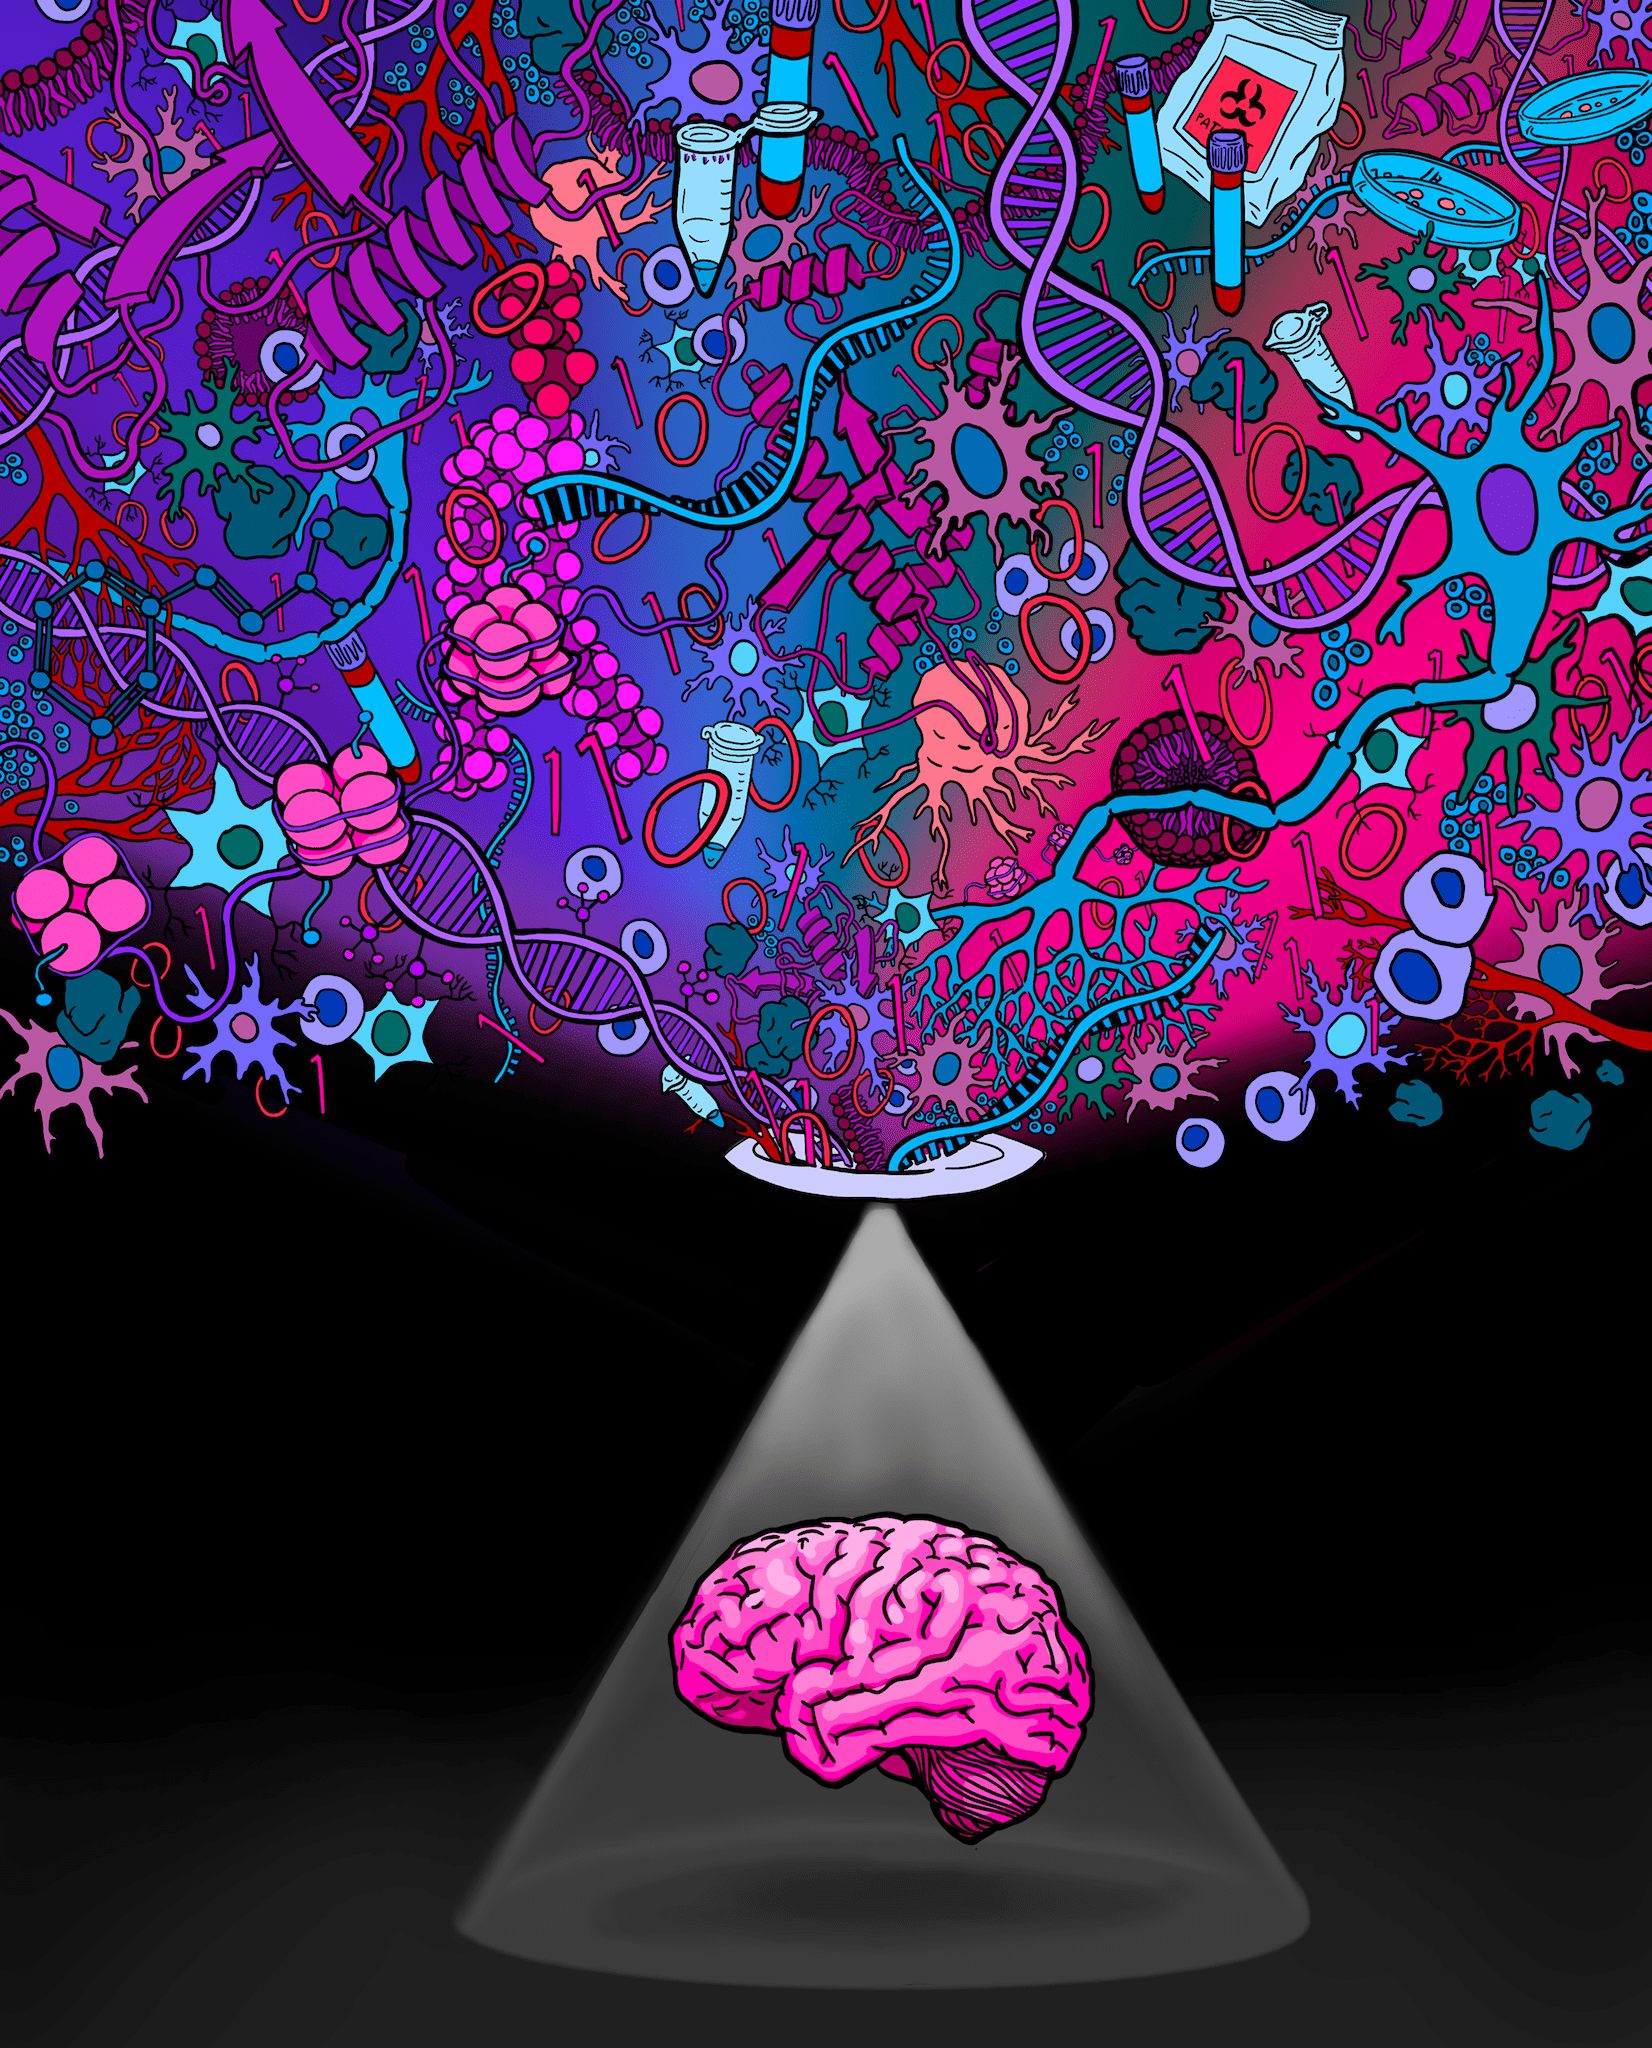
\includegraphics[width=0.6\linewidth]{figures/chap05_conclusion/cptac_gbm_cancer_cell_cover.png}
    \caption[Better disease understanding through a lens for an integrative view of multi-omics datasets.]{Better disease understanding through a lens for an integrative view of multi-omics datasets. Cover art of \textit{Cancer Cell} (April 2021 issue). Artwork by Jessica Johnson \url{https://jessicajohnsonart.com/}.}
    \label{fig:lens-multi-omics}
\end{figure}

\begin{figure}[tb]
    \centering
    \phantomlabel{fig:cptac-gbm-future-plan-longitudinal}
    \phantomlabel{fig:cptac-gbm-future-plan-heterogeneity}
    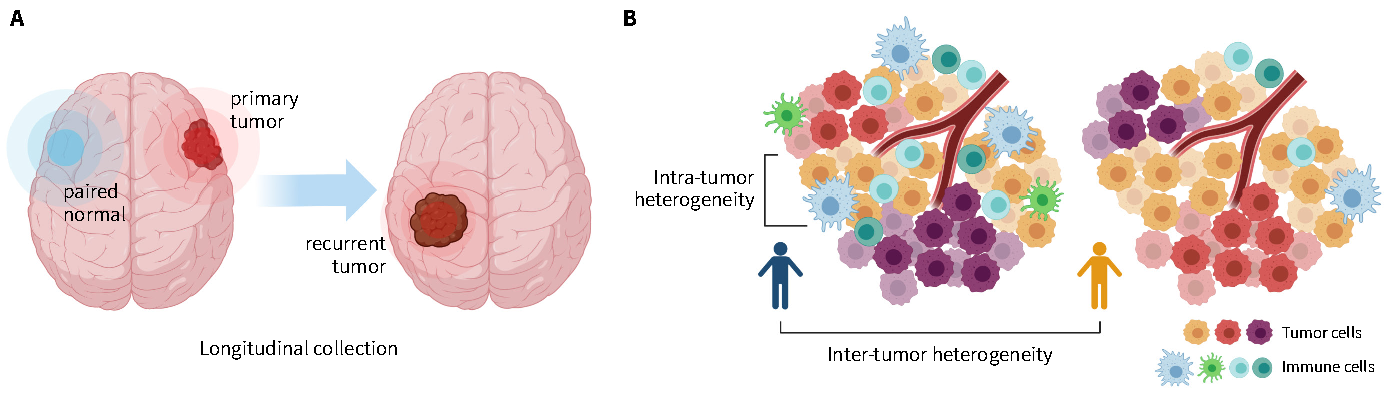
\includegraphics[width=1\linewidth]{figures/chap05_conclusion/gbm_future_plan.pdf}
    \caption[CPTAC GBM study future plan.]{%
        CPTAC GBM study future plan.
        \subref{fig:cptac-gbm-future-plan-longitudinal} Longitudinal collection of tumor samples and paired normal samples.
        \subref{fig:cptac-gbm-future-plan-heterogeneity} Tumor heterogeneity using single cell technologies.
    }
    \label{fig:cptac-gbm-future-plan}
\end{figure}
